\begin{figure}[H]
    \caption{Sistema de coordenadas de dispositivos}
    \centering
    \setlength{\tabcolsep}{0pt}
    \renewcommand{\arraystretch}{1.2}
    \begin{tabular}{
        |>{\centering\arraybackslash}m{(\textwidth - 3\arrayrulewidth) / 2}
        |>{\centering\arraybackslash}m{(\textwidth - 3\arrayrulewidth) / 2}|
    }
        \hline

        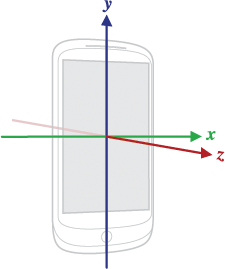
\includegraphics[width=0.4\textwidth]
        {assets/figures/second_phase/coordinate_system/img_coordinate_system_portrait.png} &
            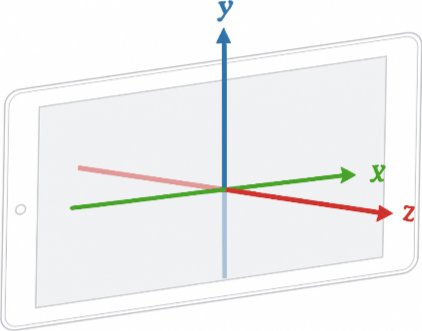
\includegraphics[width=0.4\textwidth]
        {assets/figures/second_phase/coordinate_system/img_coordinate_system_landscape.png} \\

        \small Dispositivo con orientación natural en modo retrato &
            \small Dispositivo con orientación natural en modo paisaje \\
        
        \hline
    \end{tabular}
    \caption*{\textit{Nota}. \textnormal{Imagen de modo retrato extraída de: \url{https://developer.android.com/develop/sensors-and-location/sensors/sensors_overview\#sensors-coords}}}
    \label{fig:coordinate_system_devices}
\end{figure}
\fixvspace{0.5}